José Santos y Ángel Monteagudo realizaron una serie de simulaciones en su artículo
donde intentan estudiar la influencia de los marcadores en la evolución de la simulación.
Todas las simulaciones, y sus resultados, se comentan en esta sección.

El tamaño de rejilla utilizada para todos los experimentos es de $50^3$. Esto son,
$125.000$ células posibles en la rejilla.

\section{Influencia del parámetro \textit{Tasa de mutación base (m)}}

Los autores en su artículo presentan 3 experimentos utilizando los valores por defecto
y variando el parámetro \textit{Tasa de mutación base (m)} para estudiar como afecta
dicho parámetro en la proliferación del cáncer.

Cada experimento se muestra en una serie de gráficas en las cuales se presenta
como resultado la media de 5 ejecuciones diferentes.

A continuación, se muestra cada uno de los experimentos especificando en cada caso
el valor $m$ utilizado. El resto de parámetros de la simulación se mantiene constante
con los valores considerados por defectos, que son:

\begin{table}[h!]
  \centering
  \caption{Valores de los parámetros, excepto \textit{m}.}
  \label{tab:table1}
  \begin{tabular}{ccc}
    \toprule
    Nombre & Símbolo & Valor\\
    \midrule
    Tamaño del telómero & tl & 50\\
    Muerte por daño genético & e & 10\\
    Factor de incremento de tasa de mutación base & i & 100\\
    Muerte de un vecino & g & 30\\
    Muerte aleatoria & a & 1000\\
    \bottomrule
  \end{tabular}
\end{table}

\subsection{Experimento 1: Tasa de mutación base igual a 10.000}

En este experimento, los autores obtienen una progresión lenta de las células
cancerígenas con una aparición de mutaciones similar para cada marcador, aunque
los marcadores $SG$ y $EA$ destacan frente al resto de marcadores. Por su parte,
se obtiene una alta proliferación del marcador $SG$ respecto al resto, y el marcador
$EA$ destaca levemente.

Es importante recordar, que al utilizar $1/m$ para representar la probabilidad
de que aparezcan diferentes mutaciones al realizar la mitosis, a mayor valor
del parámetro $m$, menor probabilidad de que ocurran mutaciones.

\begin{figure}[h]
\centering
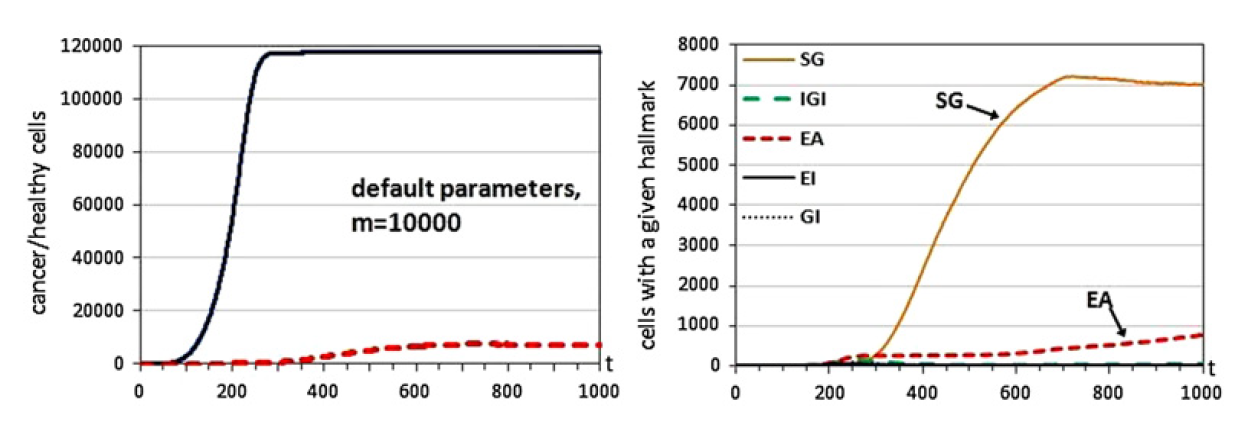
\includegraphics[scale=0.6]{figures/experiments/exp1}
\caption{Completar.}
\end{figure}

\subsection{Experimento 2: Tasa de mutación base igual a 1.000}

En este segundo experimento, los autores obtienen como resultado una mayor proliferación
de las células cancerígenas frente al experimento anterior.

Los marcadores evolucionan de forma parecida y muy homogenea, aunque destaca levemente
frente al resto el marcador $EA$.

\begin{figure}[h]
\centering
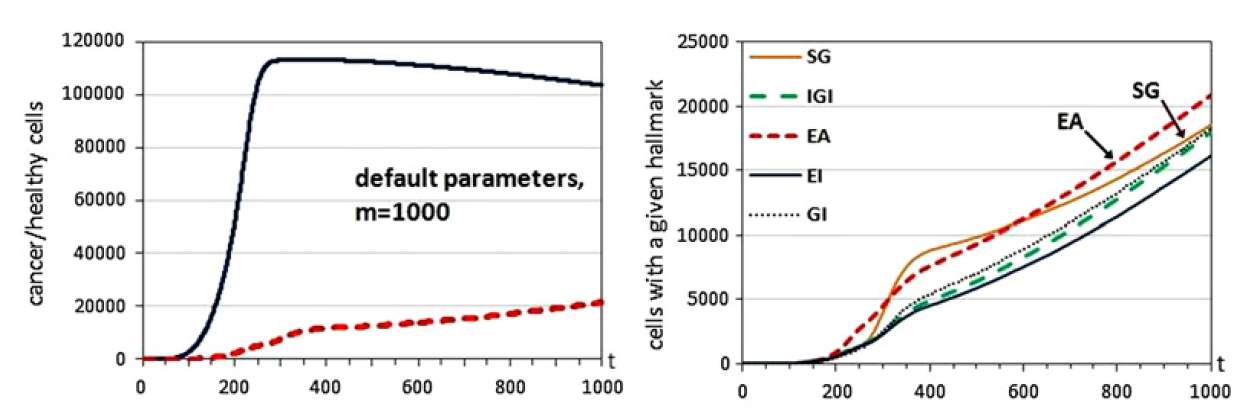
\includegraphics[scale=0.6]{figures/experiments/exp2}
\caption{Completar.}
\end{figure}

\subsection{Experimento 3: Tasa de mutación base igual a 100}

En este tercer y último experimento, los autores presentan cambios relevantes frente a los dos
experimentos anteriores.

En primer lugar, se obtiene muy pronto un mayor número de células cancerígenas
frente a células sanas, las cuales incluso decrecen.

En segundo lugar, la presencia de marcadores se mantiene de forma homogenea para todos
los marcadores, destacando levemente los marcadores $IGI$ y $EA$ frente al resto.

\begin{figure}[h]
\centering
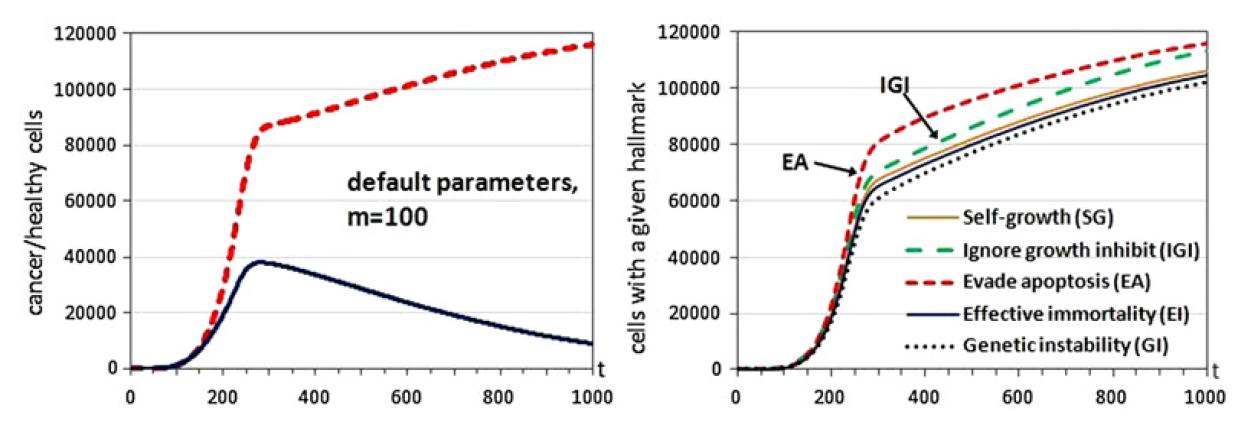
\includegraphics[scale=0.6]{figures/experiments/exp3}
\caption{Completar.}
\end{figure}

\section{Influencia del resto de parámetros}

Para observar el comportamiento del resto de parámetros, los autores, realizan una variación
de los parámetros respecto al experimento anterior. Los valores utilizados son los siguientes:

\begin{table}[h!]
  \centering
  \caption{Valores de los parámetros.}
  \label{tab:table1}
  \begin{tabular}{ccc}
    \toprule
    Nombre & Símbolo & Valor\\
    \midrule
    Tasa de mutación base & m & 100.000\\
    Tamaño del telómero & tl & 35\\
    Muerte por daño genético & e & 20\\
    Factor de incremento de tasa de mutación base & i & 100\\
    Muerte de un vecino & g & 10\\
    Muerte aleatoria & a & 400\\
    \bottomrule
  \end{tabular}
\end{table}

En este experimento, se observa como ocurre una proliferación inicial muy rápida
de células sanas, seguido de una proliferación lineal de células cancerígenas.

En cuanto a la presencia y evolución de los marcadores destaca como el marcador $EI$ hace
presencia muy pronto, y además crece muy rápidamente. El resto de marcadores presentan un
comportamiento parecido, es decir, aparecen mucho más tarde y presentan un crecimiento moderado,
destacando $EA$, el cual, presenta un crecimiento cuasi exponencial.

\begin{figure}[h]
\centering
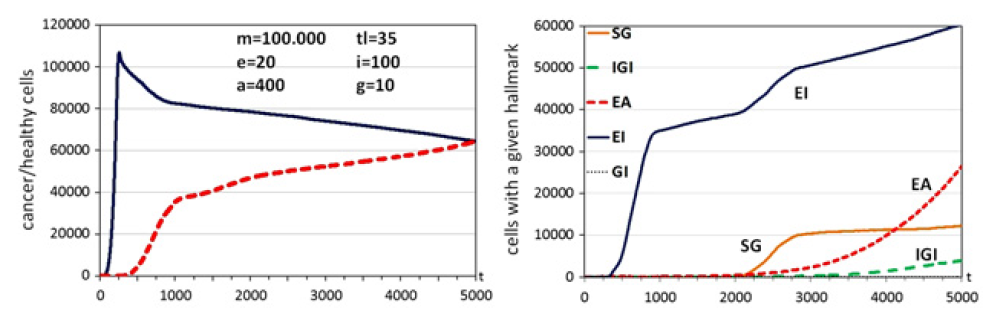
\includegraphics[scale=0.8]{figures/experiments/exp4}
\caption{Completar.}
\end{figure}

\section{Influencia de parámetros con rejilla completa de células sanas}

En este caso, se parte con una rejilla completa de células sanas. En cuanto a los parámetros,
se utilizan los mismos que en la sección anterior.

Se realizan diferentes estrategias en cuanto al número de iteraciones, desde $8000$ iteraciones
hasta $100000$ iteraciones, es decir, la simulación se corresponde con una equivalencia temporal
de $2.3$ años y $29.7$ años respectivamente.

Completar.

\begin{figure}[h]
\centering
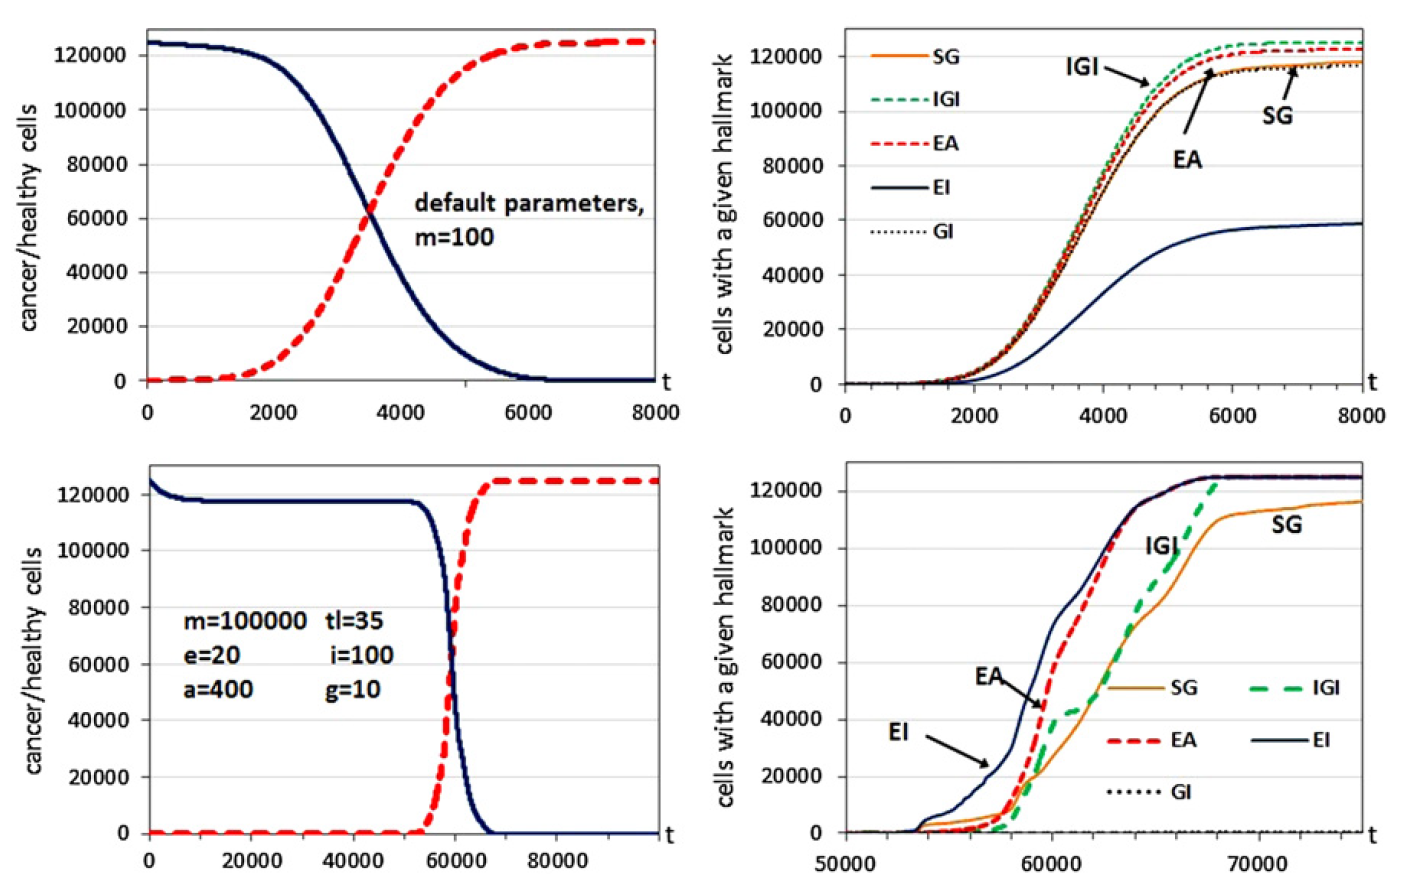
\includegraphics[scale=0.5]{figures/experiments/exp5}
\caption{Completar.}
\end{figure}

\section{Relevancia de los marcadores}

En este caso, los autores intentan responder a la siguiente pregunta: \textit{¿Cuál sería
el comportamiento emergente si algún marcador no estuviera presente y no aplicaran
sus efectos?}.

Conocer el efecto de cada marcador en el comportamiento emergente para crecimiento de tumores
puede resultar útil para mejorar las terapias contra el cáncer.

En su estudio, los autores encuentran el marcador $EA$ o de evasión de apoptosis como el más
relevante de todos, debido a que se reduce drásticamente el número de células cancerígenas.
Tras él, los siguientes marcadores más relevantes por orden son $GI$ o de inestabilidad genética y,
a continuación, $IGI$ o inhibición de señal de parada de crecimiento. Esto se debe a, en el caso
del marcador $GI$, se reducen las posibilidades de adquirir una mutación. Respecto al marcador $IGI$,
esto se debe a que cuando la rejilla no tiene espacio libre, sobre todo con células sanas, se reduce
la probabilidad de, para realizar la división, una célula mate a un vecino para conseguir espacio.

Completar.

\begin{figure}[h]
\centering
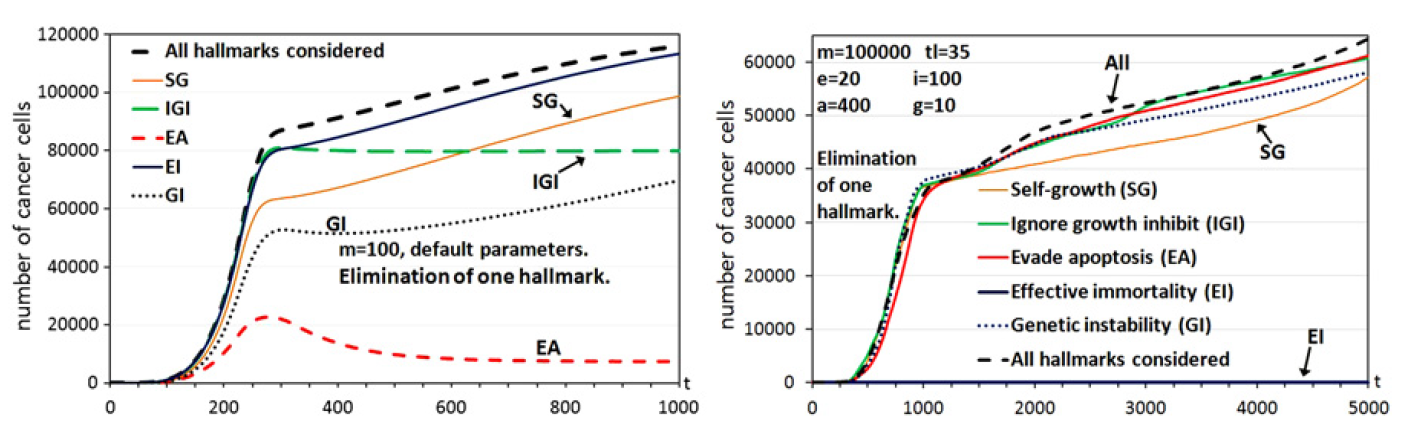
\includegraphics[scale=0.5]{figures/experiments/exp6}
\caption{Completar.}
\end{figure}

\section{Comportamiento de las transiciones}

El objetivo es estudiar el comportamiento de las transiciones cuando un agente actua contra las células cancerosas.
En este caso, la simulación comienza con la rejilla completa de células cancerosas, y se supone una terapia
perfecta, en el sentido que la droga, en este caso, actúa sólo contra las células cancerosas.

Completar.

\begin{figure}[h]
\centering
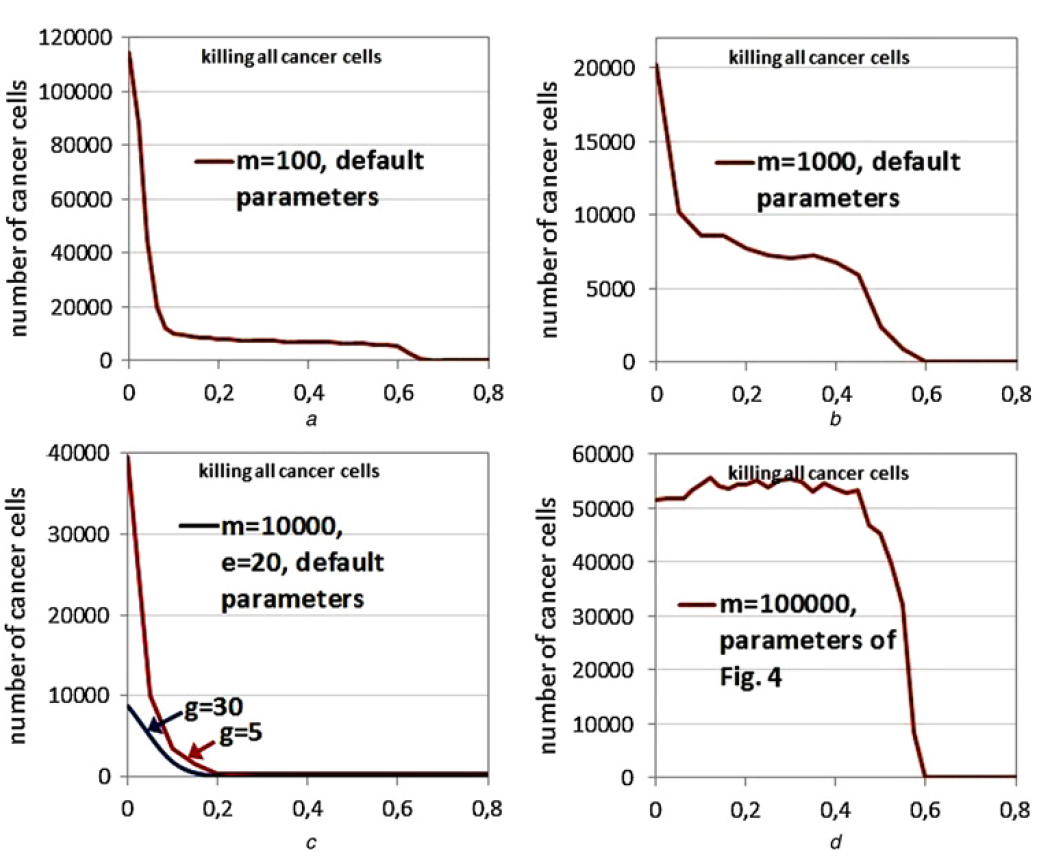
\includegraphics[scale=0.7]{figures/experiments/exp7}
\caption{Completar.}
\end{figure}

\begin{figure}[h]
\centering
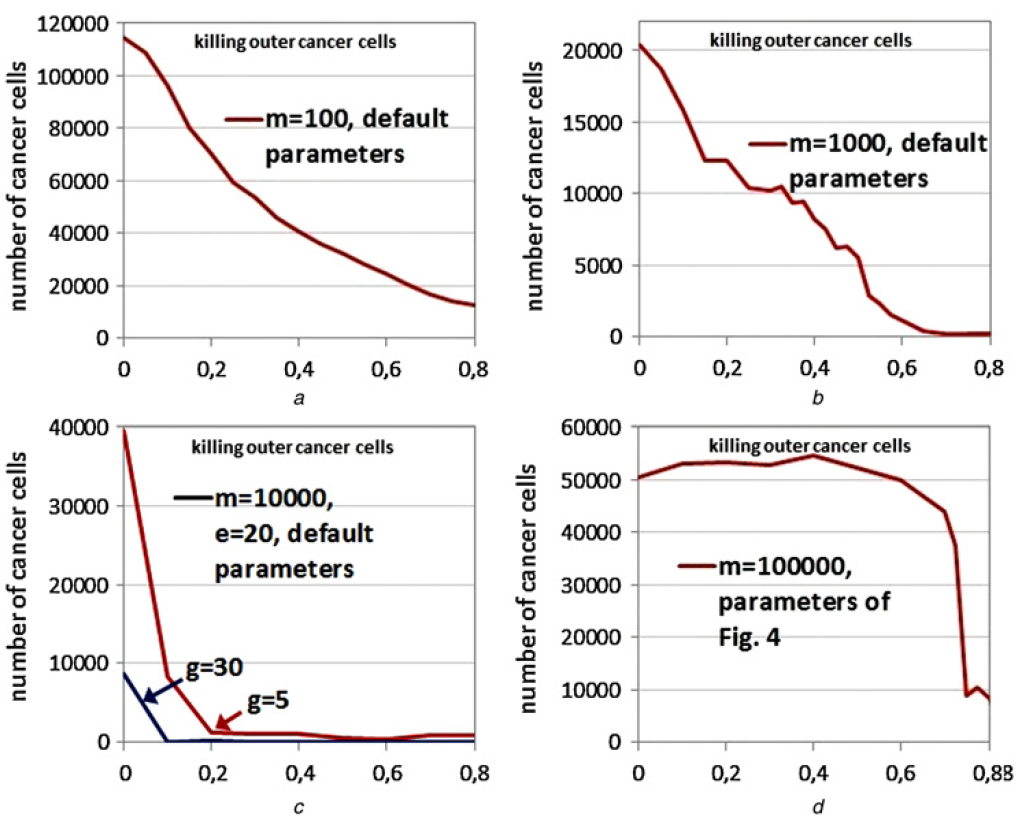
\includegraphics[scale=0.7]{figures/experiments/exp8}
\caption{Completar.}
\end{figure}
